\documentclass[12pt]{article}
\input{bayesuvius.sty}


\begin{document}
\title{Causal DAG Extraction from 3 Short Stories  \\
and 3 Movie Scripts}
\date{ \today}
\author{Robert R. Tucci\\
        tucci@ar-tiste.com}
\maketitle
\vskip2cm
\section*{Abstract}
We improve a previously proposed algorithm
for doing causal DEFT (DAG Extraction from Text), and then we apply the new algorithm to 2 usecases:
3 short stories by P.G. Wodehouse and 3 movie scripts by Pixar/Disney. The software  used to accomplish this 
endeavor is called ``Mappa Mundi" and is available as open source at GitHub. 
\newpage

\chapquote{``If humans were so good at causal inference, religion would not exist."}
{Yann LeCun}{Ref.\cite{yann-religion}}

\chapquote{``How much of human knowledge is captured in all the text ever written? To which my answer is: not much.
"}{Yann LeCun}{Ref.\cite{yann-text}}
\section{Introduction}


In this paper, I improve an algorithm
for doing causal DEFT (DAG Extraction from Text)
that was
first proposed in Ref.\cite{deft1}
I then apply the new algorithm to 2 usecases:
\begin{enumerate}

\item 3 short stories by P.G. Wodehouse
(the text from these was obtained from the
Project Gutenberg website \cite{project-gutenberg}) 

\begin{itemize}
\item  Bill the Bloodhound
\item  Extricating Young Gussie
\item Wilton's Holiday
\end{itemize}

\item 3 movie scripts by Pixar/Disney.
(the text for these was obtained from the IMSDb website Ref.\cite{imsdb})\footnote{The Mappa Mundi repo at GitHub
contains a Python script called {\tt downloading.py}
that uses the BeautifulSoup Python
package to scrape all the $1100+$ movie
scripts available (about 230 MB) at the IMSDb website.
My original intention
was to apply my algorithm to 
all of those movie scripts.
However, due to lack of
hardware resources, I had to 
settle for just 3 movie scripts.}

\begin{itemize}
\item Toy Story 
\item Up
\item WALL-E
\end{itemize}
\end{enumerate}

The Python 
software that was used to 
accomplish this endeavor is 
called Mappa Mundi. It is open source and available
at Github (Ref.\cite{github-mappa-mundi}).



So what is Mappa Mundi good for? The goal of DEFT in general and Mappa Mundi in particular is to create a directory 
of DAGs (``DAG atlas").
Conjecturing
a DAG is always the first step
in doing Judea Pearl's causal inference (CI).\footnote{Pearlian CI is described
in detail in Pearl's {\it The Book of Why}
(Ref.\cite{book-of-why})
and in my free, open source book {\it Bayesuvius} (Ref. \cite{bayesuvius}).}
Once a DAG is available,
one can use it to 
do Pearl's 3 rungs of CI.
For example, my free open source software SCuMpy (Ref.\cite{scumpy})
can be used to do all 3 rungs
of CI with linear SCM (Structural Causal Model, a type of DAG)\footnote{DAG = Directed Acyclic Graph, SCM = Structural Causal Model}, 
including
SCM with feedback loops and hidden variables. 

As I explained in my previous paper Ref.\cite{deft1}, the scientific method (SM) looks for causation, not correlation. Pearl CI is the gold standard theory for distinguishing
between correlation and causation.
Hence, the SM and CI are closely related.
CI can be viewed as an application of SM wherein the DAG is the hypothesis part of the SM, what we want to  
prove or disprove.
DEFT provides DAG hypotheses.
For example,
DEFT could be used to discover causal DAGs that indicate pathways to diseases.

At the end of this paper, I describe possible ways of improving Mappa Mundi
using LLMs (Large
Language Models such as ChatGPT).


\section{Algorithm Overview}
The algorithm proposed in this
paper can be applied to a broad range of texts. The only constraint is that those texts 
do ``story-telling" in a chronological order.
That is why I decided to use movie scripts,
because movie-scripts usually do story-telling in a chronological order (except when they do 
flashbacks or time travel, but that is fairly
uncommon in movies.)

For example, algorithm would not work well
if applied the corpus of science papers at arXiv,
because those don't do chronological story-telling. On the other hand,
it might work well if applied to a corpus of (time stamped) lab notebooks by one or more experimental scientists.
It might also work well on a corpus of time-stamped logs maintained by an individual
trying to figure out the cause of a disease 
that ails him/her.

Note also that this algorithm would
work well on a corpus of videos or movies that
do chronological story telling. This
would require that  
some human or AI
narrated the movie/video as the action happens. Such ``in-time" movie and video narration,
often referred to as AD (audio description)
(Ref.\cite{audio-description}),
and also closed captioning, are becoming 
increasingly
widespread in the movie, TV and internet video streaming industries. In certain cases, 
they are mandated by laws 
(like the CVAA, Twenty-First Century Communications and Video Accessibility Act of 2010) that
address the needs of the visually impaired.



The essence of my algorithm is simple
to describe.
Given a set of $N$ movie scripts (or short stories),
it compares all possible pairs movies.
Hence, it makes $(N^2-N)/2$
 comparisons between 2 movies.

Before comparing movies, each movie script is simplified as follows.
Each sentence is divided into clauses,
and each clause is simplified by removing
``stop-words" and other excess baggage from it.
Then we define a node of a DAG for each 
of the simplified clauses. We define
a DAG, possibly not connected, for each movie.

To compare two movies 1 and 2,
we compare every node $\tt node1$
in movie 1 with every node $\tt node2$ in movie 2.
To compare two nodes $\tt (node1, node2)$,
we use what is called, in the NLP (Natural Language Programming)
community, a {\bf similarity between two sentences}. 
If the similarity
between $\tt node1$ and $\tt node2$ exceeds a certain threshold
that we call $\tt SIMI\_THRESHOLD$,
then we store that node pair and its
similarity in a dictionary with
a node pair as key and its similarity 
as value. Call this dictionary $\tt nd1\_nd2\_bridges$.
We say that there is a {\bf bridge} 
between $\tt node1$ and $\tt node2$
if $\tt (node1, node2)$ is contained 
in the keys of $\tt nd1\_nd2\_bridges$.

\begin{figure}[h!]
\centering
\includegraphics[width=5in]
{crossing-bridges.png}
\caption{Bridges span two DAGs (i.e., movies). We consider 2 possibilities:
bridges $a$ and $b$ cross,
or they don't. 
}
\label{fig-crossing-bridges}
\end{figure}

Next we consider every  pair $\{a,b\}$
of bridges. Suppose bridge  $a$ 
connects node $\tt node1a$ in movie 1
to node $\tt node2a$ in movie 2.
Likewise, let bridge $b$ connect
$\tt node1b$ in movie 1 to
node $\tt node2b$ in movie 2.
Let $\tt node1a.time$ be the time at which 
$\tt node1a$ occurs and define
$\tt node1b.time$,
$\tt node2a.time$, and
$\tt node2b.time$ similarly.
Assume that
$\tt
node1a.time< node1b.time$.
Then there are two possibilities
that we wish to consider. These 2 possibilities are illustrated in Fig.\ref{fig-crossing-bridges}.
Either the bridges don't cross 
(i.e. $\tt node2a.time < node2b.time$)
or they cross (i.e. $\tt node2b.time < node2a.time$).\footnote{We ignore cases
where the 2 nodes in movie 1 or the 
2 nodes in movie 2 occur at the same time.}
Let $N_{rep}$ be the {\bf number
of repetitions of an arrow}.
If bridges $a$ and $b$ cross,
we do nothing.\footnote{It's also 
possible to assign a penalty
when the bridges cross,
but we don't explore that option in this paper} If they don't cross,
we do the following for both DAG1 and DAG2.
If an arrow between the earlier and latter of the two nodes doesn't already
exist, we add one with $N_{rep}=1$.
If such an arrow already exists,
we increase its $N_{rep}$ by one.

That's basically the whole algorithm.
At the end of it, we will have
generated DAG1 for movie 1 and DAG2 for movie 2.

When drawing one of those DAGs with Mappa Mundi,
one specifies a number $\tt reps\_threshold$.
Only the arrows with $N_{reps}$
larger than $\tt reps\_threshold$
are drawn.
The number $N_{reps}$ for each arrow is drawn
in the middle of the arrow.



\begin{figure}[h!]
\centering
\includegraphics[width=2in]
{shark-attacks.png}
\caption{
DAG that expresses the fact that both
shark attacks and ice
cream sales increase during the summer,
because both are caused by hot summer weather.
}
\label{fig-shark-attacks}
\end{figure}

Here is a simple argument for
why this algorithm should work.
Consider Fig.\ref{fig-shark-attacks}.
The figure depicts a DAG that
expresses the fact that both
shark attacks and ice
cream sales increase during the summer,
because both are caused by hot summer weather.
Let 

$H$ = hot summer weather starts,

$Sh$ = shark attacks increase, 

$IC$ = icream sales increase.

If we compare this DAG to $N$
other DAGs that contain these 3 nodes,
then, since it is always true
that summer precedes shark
attack increases and ice cream sales increases, the two arrows 
emanating
from the $H$ node 
will have $N_{reps} =N$.
On the other hand, we expect that half of the time, the $Sh$ node will occur before
the $IC$ node,
and half of the time it will happen after.
Hence, $N_{reps}=\frac{N}{2}$ for the
arrow $Sh\rarrow IC$.
If, when we draw this DAG, we set $\tt reps\_threshold$ to be 
greater than $\frac{N}{2}$,
then only the two causal arrows will be visible. The difference (i.e., gap) between
 $N_{reps}$ for the causal and non-causal
 arrows will grow \footnote{This gap
  can probably be made to increase
  even faster if we penalize crossing
  bridges, but 
  we won't consider that in this paper.}
   as $\frac{N}{2}$.

 

\section{Software Description}

\section{Possible Improvements
using LLMs}





\bibliographystyle{plain}
\bibliography{references}
\end{document}
